\documentclass[utf8]{article}

\usepackage[utf8]{inputenc}

\usepackage[parfill]{parskip}

\usepackage{amsmath}
\usepackage{amssymb}
\usepackage{amsfonts}
\usepackage{graphicx}
\usepackage{float}
\usepackage{listingsutf8}

\usepackage{fullpage}
\usepackage[colorlinks=true,linkcolor=black,urlcolor=blue]{hyperref}

% -----------------------------------------------------

\begin{document}

\begin{titlepage}
    \centering
    
    % Titre en haut de la page
    \vspace*{1cm}
    {\huge \bfseries Info F-201 : Projet d’OS \\
                    Rapport \par}
    
    % Espace vertical pour centrer le logo
    \vfill
    
    % Logo au milieu de la page
    \begin{figure}[h]
        \centering
        
\includegraphics[scale=0.2]{logo.png}
    \end{figure}
    
    % Espace vertical pour descendre l'auteur et la date en bas
    \vfill
    
    % Auteur et date en bas de la page
    {\large Auteurs: Liefferinckx Romain, Rocca Manuel, Radu-Loghin Rares\\ 
            Matricules: 000591790, 000596086, 000590079 \\ 
            Section: INFO \par}
    {\large 2024, 10 Novembre \par}
\end{titlepage}

\newpage
\tableofcontents

\newpage

% -----------------------------------------------------

\section{Introduction}
\subsection{Présentation du projet et contexte}
Dans le cadre de notre cours d'OS, nous avons réalisé un projet consistant à implémenter un système de chat en C.
En premier lieu, celui-ci permet la communication entre personnes via deux terminaux différents sur un même ordinateur via des pipes nommés pour la 
permettre la transmission des messages. En second lieu, la communication se fait entre un utilisateur et un script bash sobrement intitulé "chat-bot". 
Ce dernier est conçu pour simuler un utilisateur en répondant automatiquement à des commandes spécifiques envoyées par l’interlocuteur.
Donc, pour brièvement résumer, le projet se compose en deux parties : deux utilisateurs commnuiquant entre eux via un programme "chat" chacun et un utilisateur utilisant
également le programme "chat" mais pour communiquer avec le script Bash, à savoir le "chat-bot".

Ce rapport a pour but de décrire les choix d'implémentation, les difficultés rencontrées durant la conception du programme et les solutions mises en œuvre pour y remédier
le plus efficacement possible.

\subsection{Objectifs du projet}
Ce projet est le premier de cette année universitaire 2024-2025. Il possède une série d'objectifs dont voici les principaux décrits ci-dessous:
\begin{itemize}
    \item Le travail de groupe: développer des compétences collaboratives chez chaque membre et apprendre à travailler en
          équipe, même sous la pression d'une date de remise.
    \item Comprendre et appliquer les concepts théoriques vus au cours et aux TP d'OS comme la gestion d'une mémoire dynamique
          ou partagée, les processus, la communication inter-processus via des pipes nommés ou encore la gestion des signaux.
\end{itemize}

\vspace{1.5cm}
\begin{figure}[h]
    \centering
    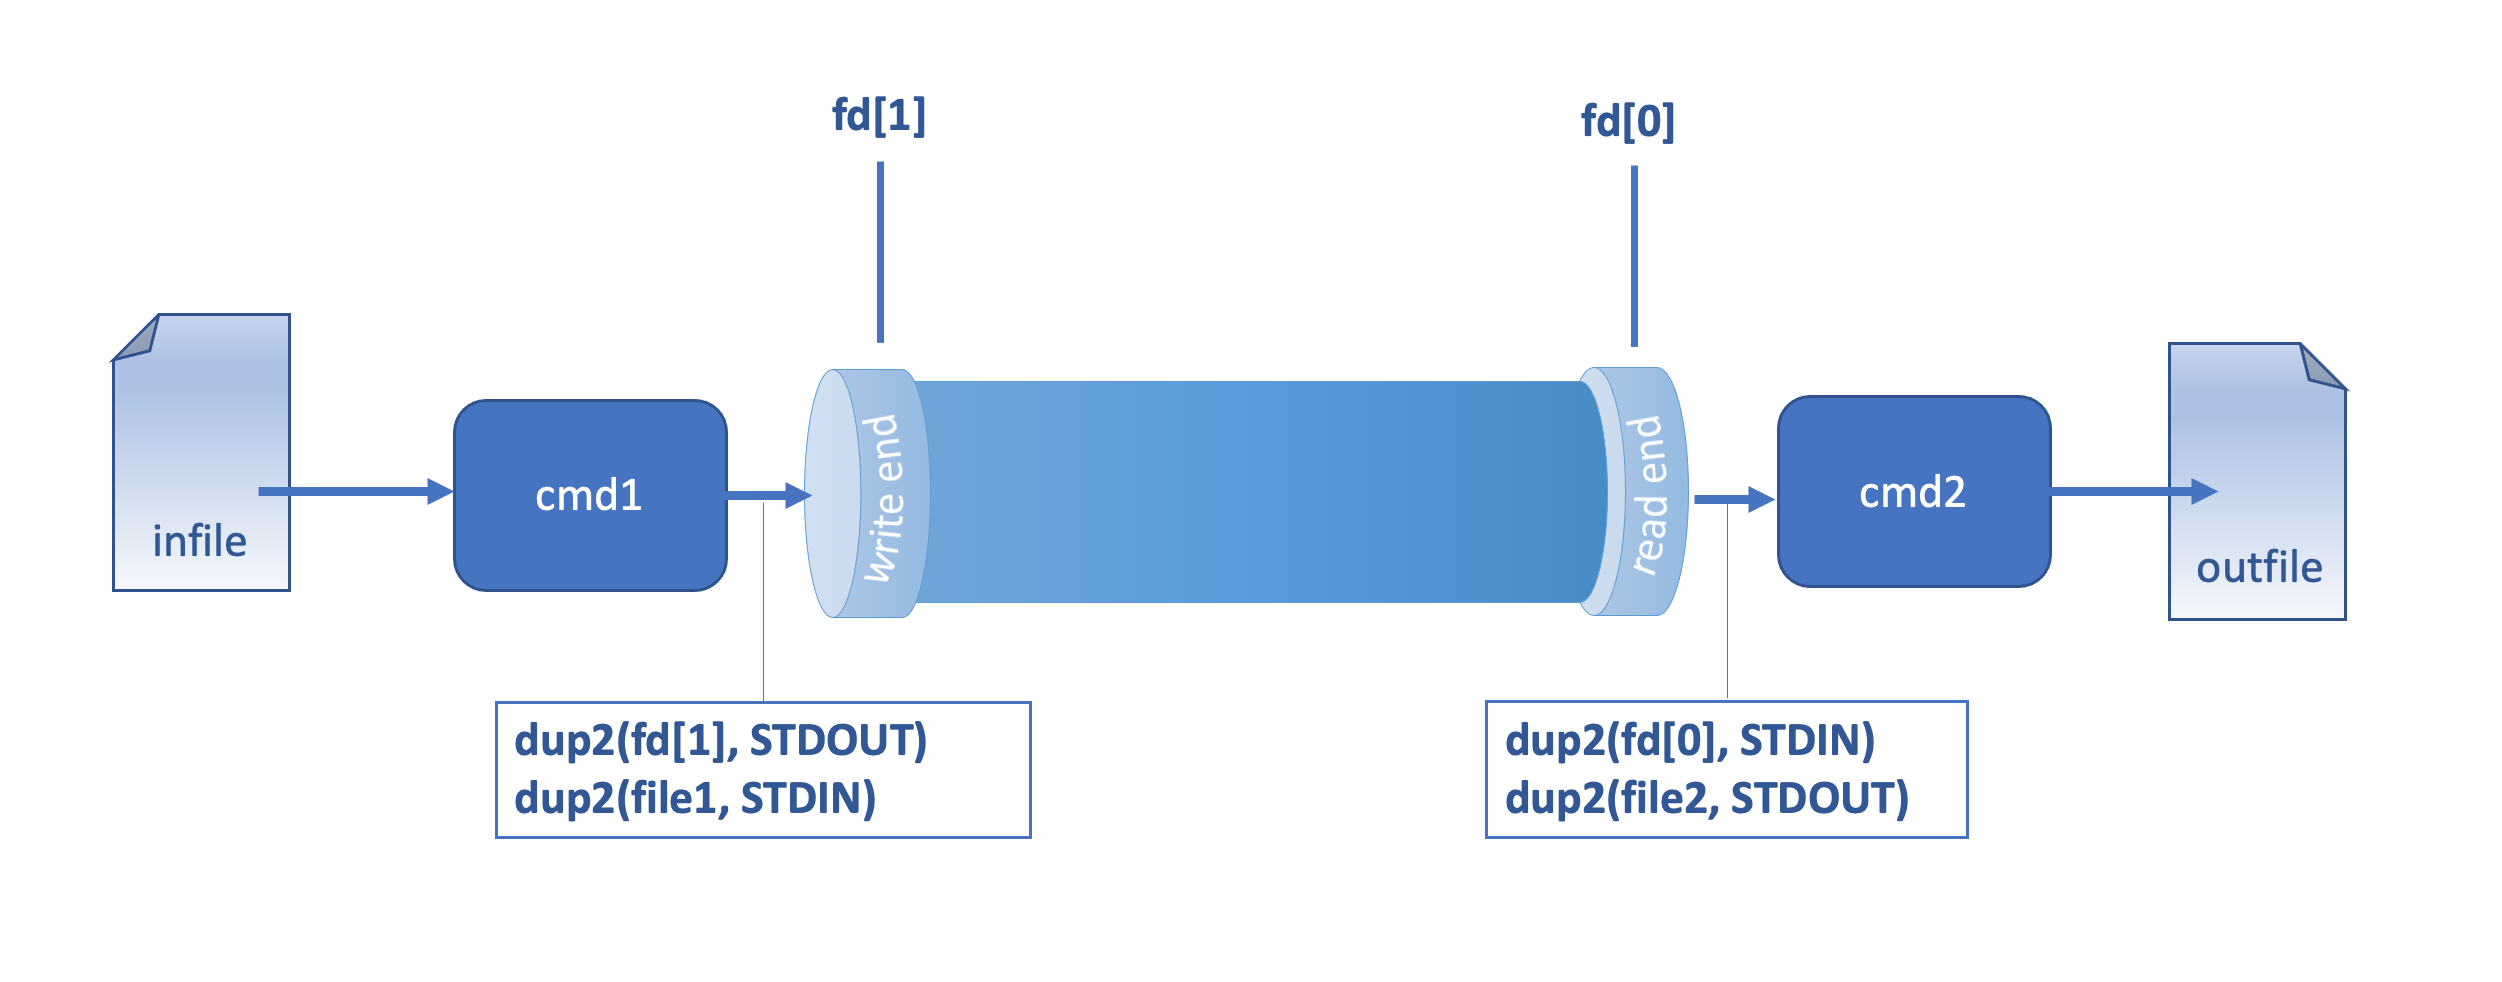
\includegraphics[scale=0.4]{pipes.png}
\end{figure}


\newpage
\section{Choix d’Implémentation}
\subsection{Choix du langage}
Pour la réalisation du projet, nous avions le choix entre deux langages de programmation, à savoir le C et le C++.
Nous avons opté pour le C car, premièrement, c'est dans ce langage que nous voyons la matière durant les séances de travaux pratiques ainsi qu'aux cours théoriques. 
Ensuite, suite à un peu de recherche, nous avons appris que les OS modernes sont majoritairement écrits en C, bien qu'ils utilisent également un peu de C++. Le langage
C tombait donc sous le sens.

\subsection{Gestion des signaux}
En ce qui concerne la gestion des processus, nous avons décidé d'utiliser la fonction "sigaction" au lieu de "signal". Celle-ci nous a été recommandée par notre assistant durant un TP
mais ce choix découle également du fait que nous avons rencontré quelques difficultés avec "signal" lors de l'implémentation du projet. Donc, "sigaction" est notre choix de fonction à utiliser pour 
gérer les signaux grâce à sa structure "struct sigaction" qui apporte une certaine modularité dans structure du code et dans la gestion des signaux. 

Cependant, dans une fraction du code (init.c, lignes 1 et 59), nous avons tout de même utilsé "signal" afin de remplacer la fonction "sigignore" en raison d'un warning à ce niveau lors de la compilation. 
En faisant nos recherches, nous sommes tombés sur cette page \href{https://stackoverflow.com/questions/36696318/handling-warning-implicit-declaration-of-function-sigignore}{StackOverflow} concernant exactement
le problème rencontré. C'est donc pourquoi nous avons décidé de remplacer "sigignore(SIGINT)" par "signal(SIGINT, SIG\_IGN)", ce qui nous a permis de régler le warning lors de la compilation.


\subsection{Gestion de la mémoire partagée}
La mémoire partagée, utilisée par le mode "--manuel", est implémentée à l'aide de la bibliothèque "mman.h" et d'une structure "sharedMemo". Cette dernière permet une gestion
par indexage de la mémoire, sans avoir à se soucier des pointeurs. Elle est donc composée d'un entier reprenant le décalage et d'un tableau de 4096 octets,
représentant la mémoire elle-même. \\En ce qui concerne son fonctionnement, nous sommes partis sur la structure de donnée "queue". Elle
permet de récupérer facilement le premier string entré grâce au principe "first-in, first-out". Nous retrouvons les fonctions pour lire et écrire, ainsi
que celles pour initialiser la mémoire et la désallouer. Une fonction permettant la lecture complète la mémoire est également mais non-utilisée, laissée à l'investigation du lecteur.
Finalement, chaque étape critique de la vie de la mémoire partagée (comme par exemple sa désallocation avec "munmap") est complémentée par de la gestion d'erreurs pour s'assurer de son bon fonctionnement.

\subsection{Communication inter-processus}
Au début nous avions fait le choix d'implémenter la communication inter-processus selon le principe suivant: le premier processus ouvre les deux fifos en mode writer et le second en mode reader.
Nous avons ensuite utilisé un fork afin que toutes les entrées soient ouvertes et que l'écriture soit possible à partir de n'importe où.
Nous avons abandonné cette approche au profit d'une autre car celle-ci empêchait le déclenchement des signaux SIGPIPE du fait que les deux entrées 
étaient ouvertes en double et que la fermeture n'était pas détectée. Au final, nous avons opté pour une ouverture du pipe d'envoi en mode écriture et le pipe de 
réception en mode lecture par le premier processus pendant que le second fait le contraire. Ainsi, nous avons une ouverture de chaque pipe permettant de détecter 
les signaux SIGPIPE sans faute.
 

\newpage
\section{Difficultés Rencontrées et Solutions}

\subsection{SIGINT et SIGPIPE}
Dans notre groupe, la première difficulté concernait la gestion des signaux avec le "SIGINT" ("Ctrl+C") et le "SIGPIPE" 
(lorsqu'un pipe est fermé), envoyés par le système d'exploitation. Selon les consignes, quand un signal est intercepté, les deux programmes 
"chat" doivent se fermer. C'est donc cette gestion de signaux qui ferment les programmes qui nous a posé problème.

Pour y remédier, nous avons décidé d'utiliser "sigaction" plutôt que "signal" comme expliqué dans la section précédente.
Les signaux sont gérés à l'aide d'une fonction signal\_management. Celle-ci est appelée à chaque fois qu'un signal est reçu.
Elle s'occupe de fermer l'entrée standard, ferme les descripteurs de fichiers, tue les processus et unlink les fifo correctement. Notons
que cette gestion se fait au cas par cas, c'est-à-dire en fonction du signal et du mode activé lors du lancement du "chat".

\subsection{Mémoire partagée}
La seconde difficulté que nous avons rencontrée concerne quant à elle la façon d'implémenter la mémoire partagée. Nous avons décidé
d'utiliser la structure "sharedMemo", expliquée plus haut, pour éviter les complications que peut apporter l'utilisation de l'arithmétique de pointeurs. En ce qui
concerne le choix de structure de donnée abstraite correspondant à nos besoin, nous avons d'abord opté pour le "stack" et son principe de "last-in, first-out", 
mais comme nous cherchons à récupérer le premier string entré, la "queue" tombait sous le sens. Expliquons brièvement notre implémentation en supposant chaîne de
caractères "str" (et en considérant l'adresse 0 de la mémoire comme la gauche): 
\begin{enumerate}
    \item Ajout de "str": elle est ajoutée en début de "queue" et le contenu déjà présent en mémoire est décalé de "strlen(str)" position vers la droite.
    \item Suppresion de "str": un simple pop suffit, l'élément le plus à droite (considérons ici "str") est retourné et l'index indiquant la fin de la mémoire 
          est diminué de "strlen(str)".
\end{enumerate}

\subsection{Taille du buffer}
Initialement, pour la taille du buffer, nous avions choisi 256 octets. Mais nous nous sommes rendu compte, en posant la question à notre assistant, 
que le buffer devait avoir une taille adaptative et potentiellement infinie. Afin de résoudre ce problème, nous nous sommes inspirés du procédé montré au premier TP de ce cours, 
c'est-à-dire une mémoire dynamique allouée avec "malloc" qui double sa taille si l'espace requis vient à être insuffisant. Nous nous sommes donc lancés sur
cette voie mais suite à quelque recherches, nous avons découvert la fonction "getline", qui récupérait un input de taille variable automatiquement et qui, de manière
générale, simplifiait le code. Nous avons tout de même laissé les fonctions initialement créées à cet effet dans le fichier "memory.c" par souci de
conservation de code fonctionnel. Elles sont laissées, une fois de plus, à l'investigation du lecteur.


\newpage
\section{Solutions Originales et Améliorations}

\subsection{Gestion des variables globales}
Comme l'orienté objet nous est inaccessible suite à notre choix du C comme langage de programmation pour le projet, nous avons dû trouver une solution
alternative aux instances de classes et leurs attributs. Notre premier réflexe fut donc d'utiliser le mot clé "const" pour expliciter quelle variable peut
être modifiée et quelle variable ne peut pas l'être. Mais une deuxième option s'offrait à nous: "\#define". Celle-ci apporte une 
lisibilité accrue, et permet d'économiser de l'espace mémoire (grâce au préprocesseur qui remplace toutes les occurrences du nom défini par sa valeur avant 
la compilation du programme). Des problèmes de compatibilité entre types pourraient apparaître, certes, mais nous n'utilisons les variables 
globales en tant que types simples comme "int" ou "str", tout en faisant attention à leur contexte d'utilisation, nous permettant ainsi d'éviter les erreurs.

Afin d'obtenir une structure avec le plus de clarté possible dans notre projet, nous avons créé des fichiers "global.h" et "constant.h" pour éviter les déclarations
multiples de variables globales dans différents fichiers à la fois.

\subsection{Amélioration du script bash "chat-bot"}
Étant nouveaux au bash scripting, nous avons d'abord écrit le code bash en une traite, sans l'utilisation de fonctions. Cela donnait une impression de
code brouillon possédant peu de clarté. C'est pourquoi vers la fin du projet, nous avons pris le temps de nous repencher dessus et de refactorer le code à l'aide
de fonctions pour plus de clarté.

Nous souhaitons également souligner que nous avons découvert des memory leaks lorsque le script "chat-bot" se fermait soudainement suite à une erreur (par exemple, arrêt du
script lorsqu'une mauvaise commande est entrée). Par déduction, nous sommes arrivés à la conclusion que ce leak provenait des pipes qui n'étaient pas désalloués correctement
en fin de programme. Pour y remédier, nous avons créé la fonction "cleanUp", appelée en fin de script, qui a pour but de fermer les pipes proprement. Nous avons également pensé
à mettre un "wait" pour attendre la fin des processus concernés afin que les pipes soient vidés de leur contenu avant de les fermer, mais suite a du testing, nous n'en n'avons pas
vu l'utilité malgré le fait que c'est une bonne pratique (c'est d'ailleurs pour cela que nous le soulignons ici).

\begin{figure}[H]
    \centering
    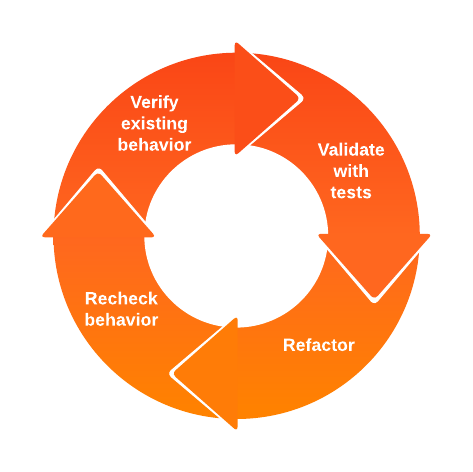
\includegraphics[scale=0.4]{refactoring.png}
\end{figure}


\newpage
\section{Conclusion}
Ce projet nous a permis de mettre en pratique et de se familiariser avec les concepts vus en cours d'OS, tels que la gestion des processus, des signaux, la gestion 
de la mémoire partagée, et la communication inter-processus en C. En faisant usage d'outils de programmation comme sigaction, fork ou encore les pipes nommés, nous 
avons découvert un nouvel aspect du vaste monde qu'est l'informatique tout en créant quelque chose par la même occasion. Sur la plan humain, ce fut une expérience courte
mais marquante car, en contraste avec nos projets de première année de bachelier qui se faisaient seuls, nous avons eu l'occasion de le faire à deux ou trois membres, au 
choix ou non. Ceci impliquait certains avantages comme la répartition de tâches permettant à chaque membre d'avoir une charge de travail réduite, mais également d'autres 
aspects pas toujours positifs, comme la gestion d'équipe, qui peut parfois s'avérer laborieuse avec une limite de temps qui approche de jour en jour. Heureusement, cette 
gestion s'est faite sans accrocs dans notre groupe et nous a permis d'avoir un aperçu réaliste des exigences du travail en équipe dans le monde professionnel.


\end{document}
